%%%%%%%%%%%%%%%%%%%%%%%%%%%%%%%%%%%%%%%%%%%%%%%%%%%%%%%%%%%%%%%%%%%%%%%
%% Document: Thesis for PhD at UC Riverside                          %%
%% Description: A comparative analysis of environment sensing in EDF %%
%% Author: Steven Ahrendt                                            %%
%%%%%%%%%%%%%%%%%%%%%%%%%%%%%%%%%%%%%%%%%%%%%%%%%%%%%%%%%%%%%%%%%%%%%%%
% INHIBITION FIGURES %
%%%%%%%%%%%%%%%%%%%%%%
\begin{figure}[hb]
  \centering
  \includegraphics[width=4in]{./Chapter_Inhibition/img/Nc_HpBdSp_otherChytrids.png}
  \caption[Inhibition appears unique to \textit{Hp} among other chytrids.]{\textit{Batrachochytrium dendrobatidis} JEL 423 (\textit{Bd}), the closest relative of \textit{Hp}, is well known as a global emerging pathogen of amphibians and is the causative agent for recent worldwide amphibian decline. \textit{Spizellomyces punctatus} SW-1 (\textit{Sp}) is a soil saprobe and is not known to be pathogenic. A) \textit{Hp} cultured with \textit{N. crassa} produces a cleared zone. B) \textit{Bd}, C) \textit{Sp}, D) \textit{Operculomyces laminatus} JEL 223, E) \textit{Rhizoclosmatium hyalinus} JEL 800, F) \textit{Obelidium mucronatum} JEL 802 do not display this property. Black scale bars = 1mm. Black arrowheads illustrate location of chytrid sporangia.}
  \label{fig:ChInhib_NcraChytrid}
\end{figure}

\begin{figure}[hb]
  \centering
  \includegraphics[width=4in]{./Chapter_Inhibition/img/HpvsOtherFungi.png}
  \caption[Inhibition is not specific to \textit{N. crassa}.]{A selection of fungal species from the Ascomycota, Basidiomycota, and Mucorales were assayed for sensitivity against \textit{Hp} sporangia. A) \textit{Neurospora crassa} (Sordariomycetes; Sordariales; Sordariaceae), B) \textit{Neurospora tetrasperma}, C) \textit{Neurospora discreta}, D) \textit{Trichoderma reesei} (Sordariomycetes; Hypocreales; Hypocreaceae), E) \textit{Aspergillus nidulans} (Eurotiomycetes; Eurotiales; Trichocomaceae), F) \textit{Coprinopsis cinerea} (Agaricomycetes; Agaricales; Psathyrellaceae), G) \textit{Ashbya gossypii} (Saccharomycetes; Saccharomycetales; Saccharomycetaceae), H) \textit{Phycomyces blakesleeanus} (Mucorales; Phycomycetaceae), and I) \textit{Rhizopus oryzae} (Mucorales; Mucoraceae). Scale bars for A-C,H-I = 1mm. Scale bars for D-G = 5mm. Black arrowheads in A-C,H-I indicate \textit{Hp} sporangia. White arrowheads in A-G indicate blocks of agar with active \textit{Hp} sporangia.}
  \label{fig:ChInhib_HpOtherFungi}
\end{figure}

\begin{figure}[hb]
  \centering
  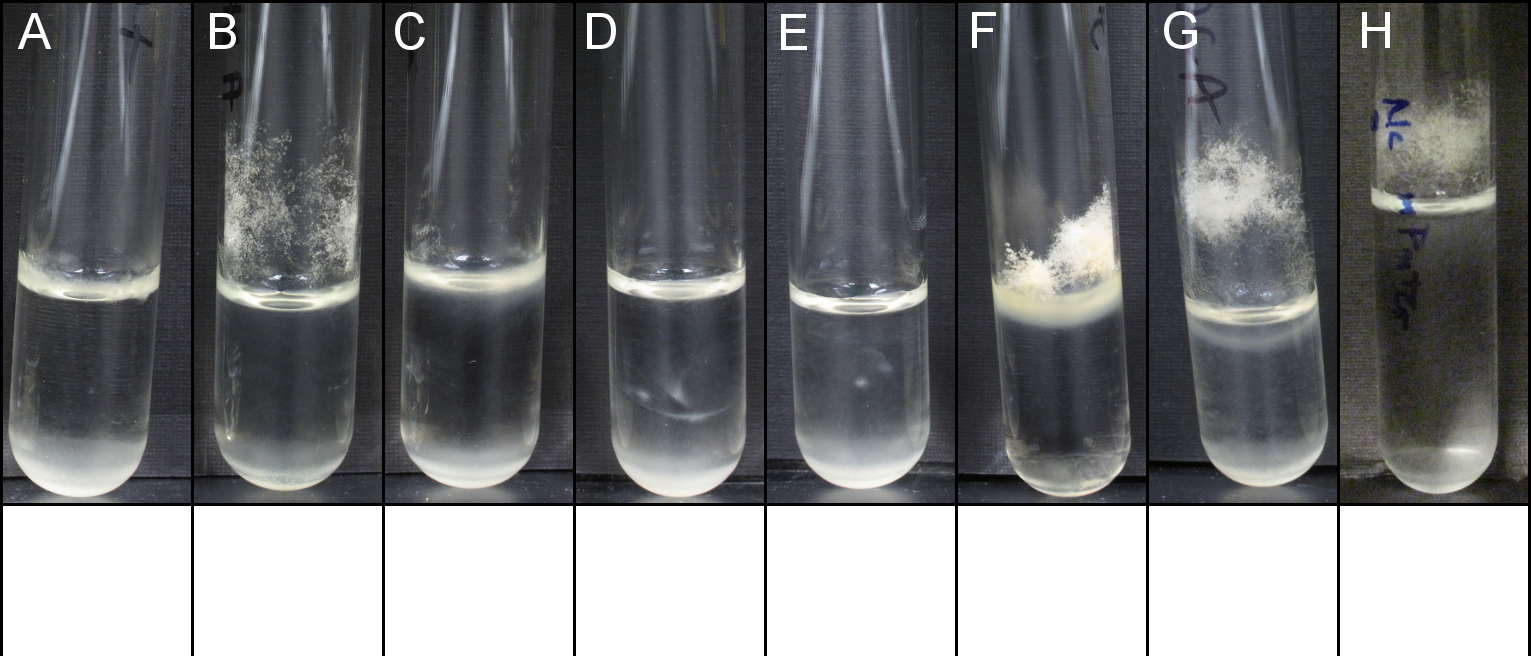
\includegraphics[width=4in]{./Chapter_Inhibition/img/96h_HpNcColdHotFresh.png}
  \caption[Conditioned media inhibits \textit{N. crassa} growth.]{Test tubes containing filter-sterilized \textit{Hp}-conditioned media ("filtrate") were inoculated with \textit{N. crassa} conidia and left to incubate at room temperature for 96h (see methods for more detail). For A), B), and C), filtrate was derived from initial preparations of \textit{Hp} alone, \textit{N. crassa} alone, and \textit{Hp}+\textit{N. crassa}, respectively. Panel B) establishes that nutrient limitation is not responsible for inhibitory observation as growth of \textit{N. crassa} can still be supported, while A) and C) establish that \textit{Hp} is not exhibiting this behavior as a response to the presence of another fungus. D), E), F), G) contain \textit{Hp}-derived mPmTG filtrate after low (-20$^{\circ}$C), high (60$^{\circ}$C), ultra-low (-80$^{\circ}$) and ultra-high (90$^{\circ}$) temperature treatments, respectively. For D-G, N. crassa inoculation occurred after media was allowed to return to room temperature. H) \textit{N. crassa} growth in fresh mPmTG media.}
  \label{fig:ChInhib_FilterTempAssay}
\end{figure}

\begin{figure}[hb]
  \centering
  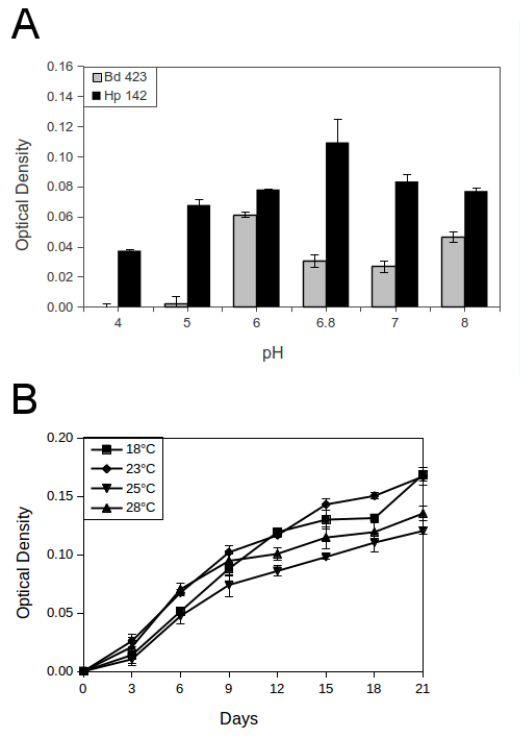
\includegraphics[width=4in]{./Chapter_Inhibition/img/HpBd_pHTempAssay.png}
  \caption[\textit{Hp} is more tolerant of environmental stresses than \textit{Bd}.]{A) \textit{Hp} and \textit{Bd} were grown at different pH levels, ranging from 4 to 8. A pH of 6.8 represents the standard pH at which the respective optimal media is prepared. B) \textit{Hp} growth after x days at various temperatures ranging from y$^{\circ}$C to z$^{\circ}$C.}
  \label{fig:ChInhib_HpBdpHTemp}
\end{figure}

\begin{figure}[hb]
  \centering
  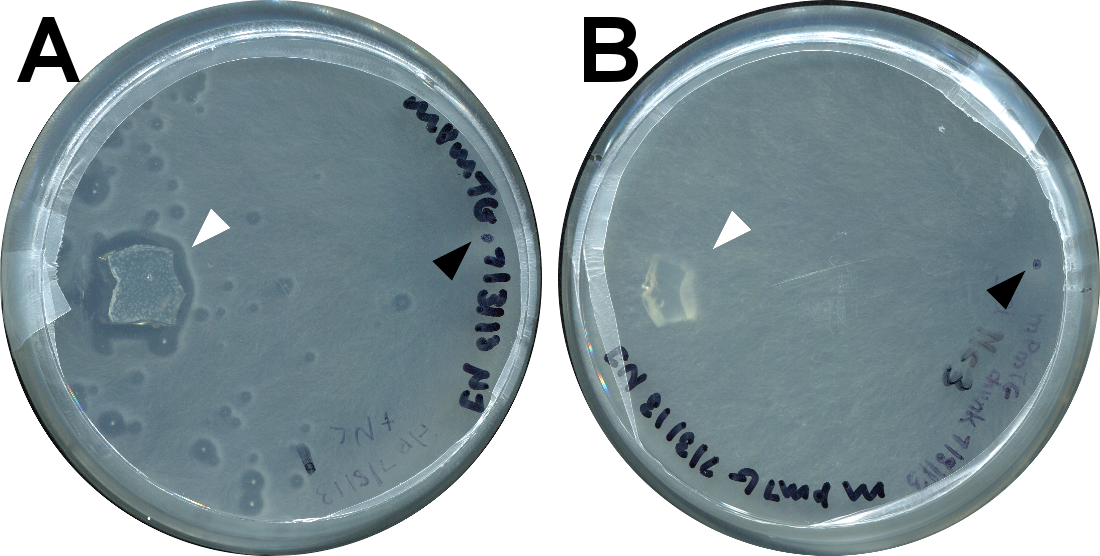
\includegraphics[width=4in]{./Chapter_Inhibition/img/HpNc_avoidance.png}
  \caption[\textit{N. crassa} displays no avoidance behavior of solid agar blocks.]{Solid agar plates of mPmTG media containing A) actively growing \textit{H. polyrhiza} and B) no \textit{H. polyrhiza} growth. After 72 hours post-inoculation of \textit{N. crassa}, zones of inhibition are clearly visible surrounding \textit{H. polyrhiza} sporangia. White arrowheads in A and B indicate agar blocks containing or lacking, respectively, \textit{H. polyrhiza} sporangia. Black arrowheads indicate point of inoculation with \textit{N. crassa} conidia. Plates are 100mm in diameter.}
  \label{fig:ChInhib_NcAvoidance}
\end{figure}

%\begin{figure}[hb]
%  \centering
%  \includegraphics[width=4in]{./Chapter_Inhibition/img/Liquid_96hAssay.png}
%  \caption[Liquid 96h assay.]{Hp conditioned media filtrate loses its efficacy after around 96h at room temperature. A) Conditioned media derived from “Hp alone” preparations. B) Conditioned media derived from “Hp+Nc” preparations.}
%  \label{fig:Liquid_96h}
%\end{figure}

\begin{figure}[hb]
  \centering
  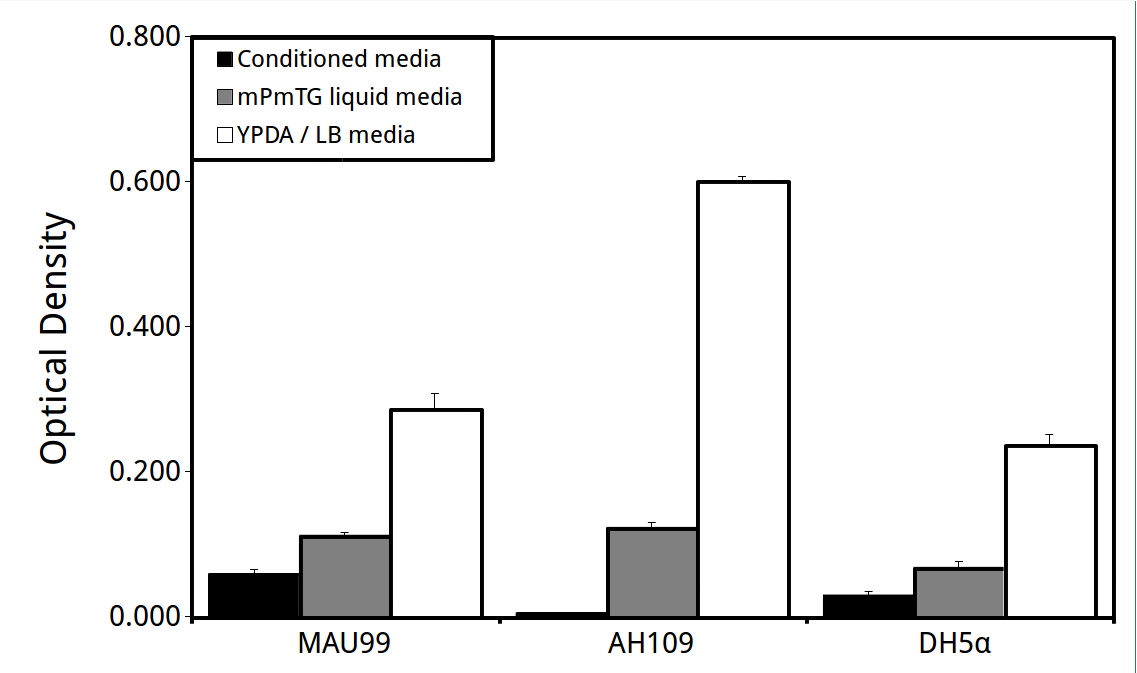
\includegraphics[width=4in]{./Chapter_Inhibition/img/yeastEcoli_liqGrowth.png}
  \caption[\textit{S. cerevisiae} and \textit{E. coli} liquid cultures are inhibited by \textit{Hp} conditioned media.]{OD$_{600}$ measurements of liquid cultures of \textit{S. cerevisiae} MAU99 and AH109, and \textit{E. coli} DH5$\alpha$ after 72h stationary incubation in different media preparations at room temperature: filter-sterilized \textit{Hp}-conditioned media (black), \textit{Hp} liquid mPmTG media (grey), and either liquid YPDA or LB for yeast or \textit{E. coli}, respectively (white).}
  \label{fig:ChInhib_HpYeastEcoli}
\end{figure}

%\begin{figure}[hb]
%  \centering
%  \includegraphics[width=4in]{./Chapter_Inhibition/img/Ncra_liquidDilution.png}
%  \caption[\textit{N. crassa} remains susceptible to \textit{H. polyrhiza} conditioned media after dilution]{Filter-sterilized \textit{Hp} conditioned media ("filtrate") was diluted to A) 100\%, B) 50\%, C) 20\% , D) 10\%, and E) 0\% with mPmTG and sterile diH$_{2}$O.}
%  \label{fig:ChInhib_NcraDilution}
%\end{figure}

%\begin{figure}[hb]
%  \centering
%  \includegraphics[width=4in]{./Chapter_Inhibition/img/030915_BdmPmTG_BdFiltrate_on1T_14d.png}
%  \caption[Incubation in \textit{H. polyrhiza} conditioned media prevents encystment and subsequent growth of \textit{B. dendrobatidis} zoospores]{Filter-sterilized \textit{Hp} conditioned media ("filtrate") was used as a growth medium for \textit{B. dendrobatidis} sporangia-containing agar blocks. After a 72hour incubation at room temperature, the liquid suspension was removed and plated on 1\% Tryptone agar plates. Plates were examined after 14d room temperature incubation. Zoospore suspensions were drawn from A) filtrate preparations and B) fresh mPmTG preparations.}
%  \label{fig:ChInhib_HpvsBd}
%\end{figure}
